% !TEX program = xelatex

\documentclass[10pt,a4paper]{article}
\usepackage[top = 1.5cm, bottom = 1.5cm, left = 1.5cm, right = 1.5cm]{geometry}

\usepackage{titling}
\usepackage[czech]{babel}
\usepackage{graphicx}
\usepackage{lmodern}
\usepackage{hyperref}
\usepackage{setspace}
\usepackage{csvsimple}

\usepackage{amsmath}
\usepackage{amssymb}
\usepackage{gensymb}
\usepackage{mathtools}
\usepackage{units}
\usepackage{bm}
\delimitershortfall=-1pt

\usepackage{gnuplottex}
\usepackage{epstopdf}

% no page break
\newenvironment{absolutelynopagebreak}
  {\par\nobreak\vfil\penalty0\vfilneg
   \vtop\bgroup}
  {\par\xdef\tpd{\the\prevdepth}\egroup
   \prevdepth=\tpd}


% redefine \sqrt
\usepackage{letltxmacro}
\makeatletter
\let\oldr@@t\r@@t
\def\r@@t#1#2{%
\setbox0=\hbox{$\oldr@@t#1{#2\,}$}\dimen0=\ht0
\advance\dimen0-0.2\ht0
\setbox2=\hbox{\vrule height\ht0 depth -\dimen0}%
{\box0\lower0.4pt\box2}}
\LetLtxMacro{\oldsqrt}{\sqrt}
\renewcommand*{\sqrt}[2][\ ]{\oldsqrt[#1]{#2\,}\,}
\makeatother

\DeclarePairedDelimiter\ceil{\lceil}{\rceil}
\DeclarePairedDelimiter\floor{\lfloor}{\rfloor}

\AtBeginDocument{\renewcommand*{\hbar}{{\mkern-1mu\raisebox{-0.055em}{$\mathchar'26$}\mkern-8mu\mathrm{h}}}}

\def\ph{\phantom}
\def\vph{\vphantom}
\def\hph{\hphantom}

\def\?{\mathit{?}}

\newcommand{\comm}[2]{\left[ #1, #2 \right]}
\newcommand{\const}[1]{\text{#1}}
\newcommand{\norm}[1]{\left\lVert#1\right\rVert}

\newcommand{\mat}[1]{
    \begin{pmatrix}
        #1
    \end{pmatrix}
}

\newcommand{\mata}[2]{
    \left(
    \begin{array}{@{}#1@{}}
        #2
    \end{array}
    \right)
}

\newcommand{\smat}[2][1]{
    \scalebox{#1}{$\mat{#2}$}
}

\renewcommand{\d}[1]{\;\const{d}#1}
\newcommand{\dd}[2]{\frac{\const{d} #1}{\const{d} #2} \;}
\newcommand{\pd}[2]{\frac{\partial  #1}{\partial  #2} \;}

\newcommand{\bra}[1]{\left< #1 \right|}
\newcommand{\ket}[1]{\left| #1 \right>}
\newcommand{\braket}[2]{\left< #1 \middle| #2 \right>}

\newcommand{\e}[1]{\const{e}^{#1}}
\renewcommand{\i}{\const{i}}

\begin{document}

\title{Kvantová mechanika I: Domácí úkoly}
\author{Michal Grňo}
\date{\today}

\maketitle

\section{Cvičení 20. 11.}

\subsection{Zadání}
Máme částici v potenciálu daném vztahem
\begin{gather*}
    V(x) = \sum_{n=-\infty}^\infty \delta(x-na).
\end{gather*}
Pro kladné energie je podle Blochova teorému vlnová funkce pro $na < x < (n+1)a$:
\begin{gather*}
    \psi_q(x) = \left( A \e{\i k (x-na)} + B \e{-\i k (x-na)} \right)\e{\i q n a},
\end{gather*}
kde $q$ je krystalová hybnost částice. Vztah energie a hybnosti je
\begin{gather}
    \cos qa = \cos ka + \frac{K}{2k} \sin ka,
    \label{implicitni-qE}
\end{gather}
\begin{gather*}
    k = \frac{1}{\hbar} \sqrt{2ME},
    \hspace{2em}
    \floor*{\frac{ka}{\pi}} = \floor*{\frac{qa}{\pi}},
\end{gather*}
kde $M$ je hmotnost částice.

Pro kladnou energii vykreslete grafy $E(q)$, $v_\const{g}(q)$, $v_\const{g}(E)$ pro $K=10$ a $K=1$. Vypočtěte normalizovanou vlnovou funkci odpovídající záporným energiím a vykreslete pro ni graf $E(q)$ pro $K=-10$ a $K=-1$.


\subsection{Řešení pro $E>0$}
Implicitní vztah mezi $q$ a $E$ chceme nějak parametrizovat. Nejprve si zadefinujeme pomocnou funkci
\begin{gather*}
    \theta_K(t) = \cos(2\pi t) + \frac{aK}{4\pi t} \sin(2\pi t).
\end{gather*}
Je zřejmé, že se jedná o pravou stranu rovnice \eqref{implicitni-qE} po substituci $ka=2\pi t$. Je snadné vyjádřit vztah mezi parametrem $t$ a energií. V dalším budeme používat „redukovanou“ energii, vydělenou konstantami:
\begin{gather*}
    \tilde{E}(t) = \frac{E}{\mathrm{h}^2 M^{-1}} = \frac{t^2}{2a^2},
    \hspace{2em}
    t(\tilde{E}) = a \sqrt{2\tilde{E}}.
\end{gather*}
Nyní si vyjádříme $q$ v závislosti na parametru. Je třeba věnovat pozornost správné volbě správné větve $\arccos$, aby byla splněna podmínka $\floor{ka/\pi} = \floor{qa/\pi}$. Lze snadno ověřit, že následující vztah tuto podmínku splňuje:
\begin{gather*}
    q_K(t) = \begin{cases}
        n \leq t \leq n + \frac{1}{2}: \;
        \frac{1}{a} \left( 2\pi n + \arccos \theta_K(t) \right)
        \\[5pt]
        n - \frac{1}{2} \leq t \leq n: \;
        \frac{1}{a} \left( 2\pi n - \arccos \theta_K(t) \right)
    \end{cases}
    \;\;
    \text{pro nějaké } n \in \mathbb{Z}
\end{gather*}
Nyní máme hotovou parametrizaci $\varphi(t)$ grafu $\tilde{E}(q)$:
\begin{gather*}
    \varphi(t) = \mat{
        q_K(t) \\[8pt]
        \tilde{E}(t)
    },
\end{gather*}
a můžeme vykreslit grafy pro první čtyři energetické hladiny (tj. $t \in [-4, 4]$).

\begin{figure}[p]
    \centering
    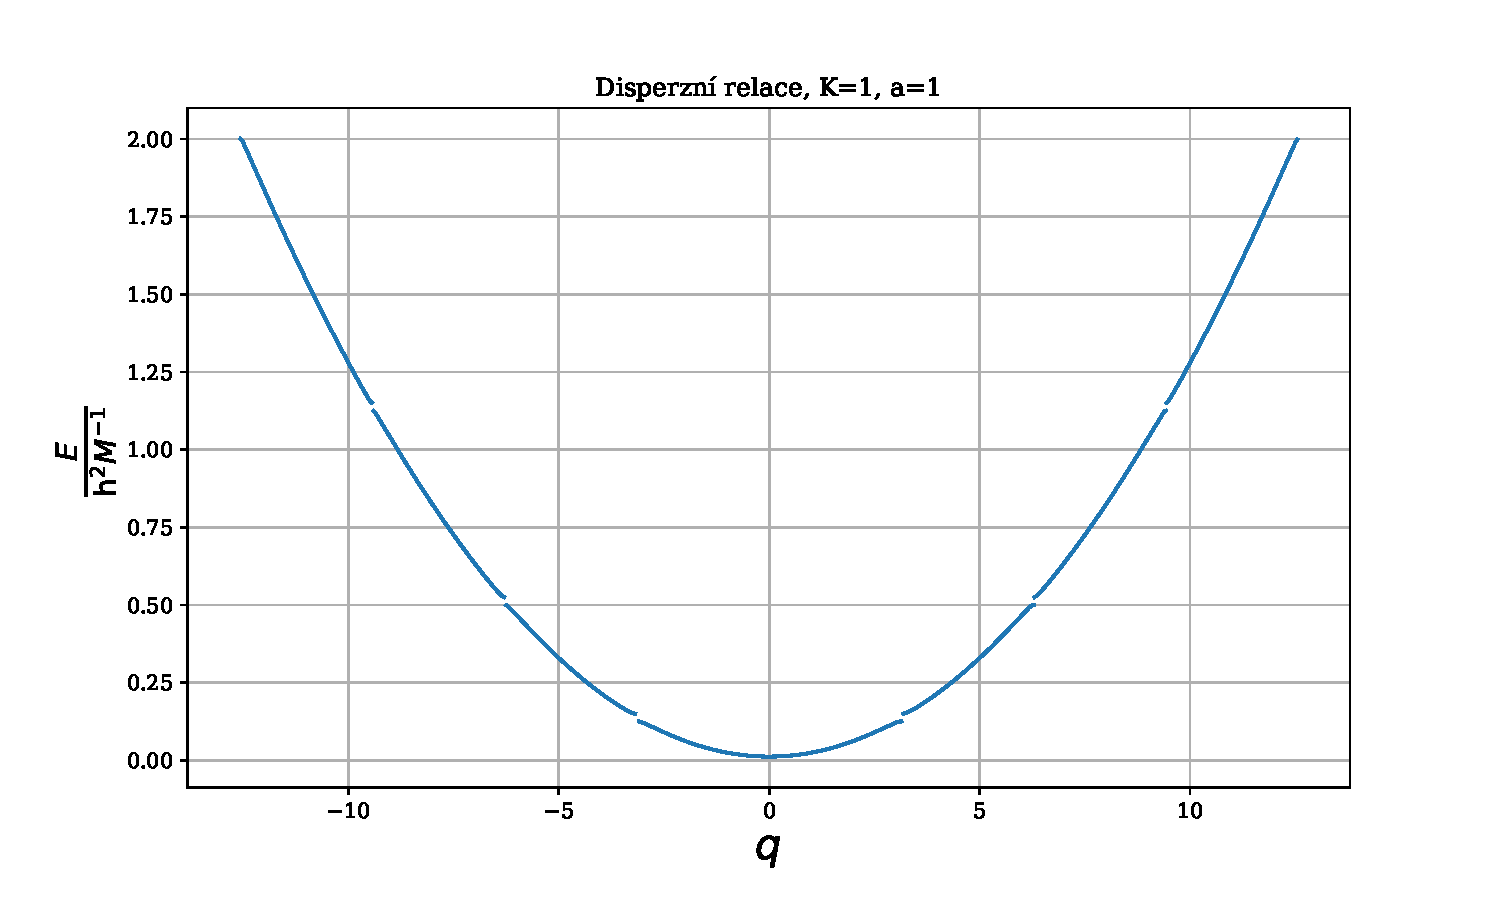
\includegraphics[scale=0.7]{disperzni1.pdf}
    \label{}
\end{figure}

\begin{figure}[p]
    \centering
    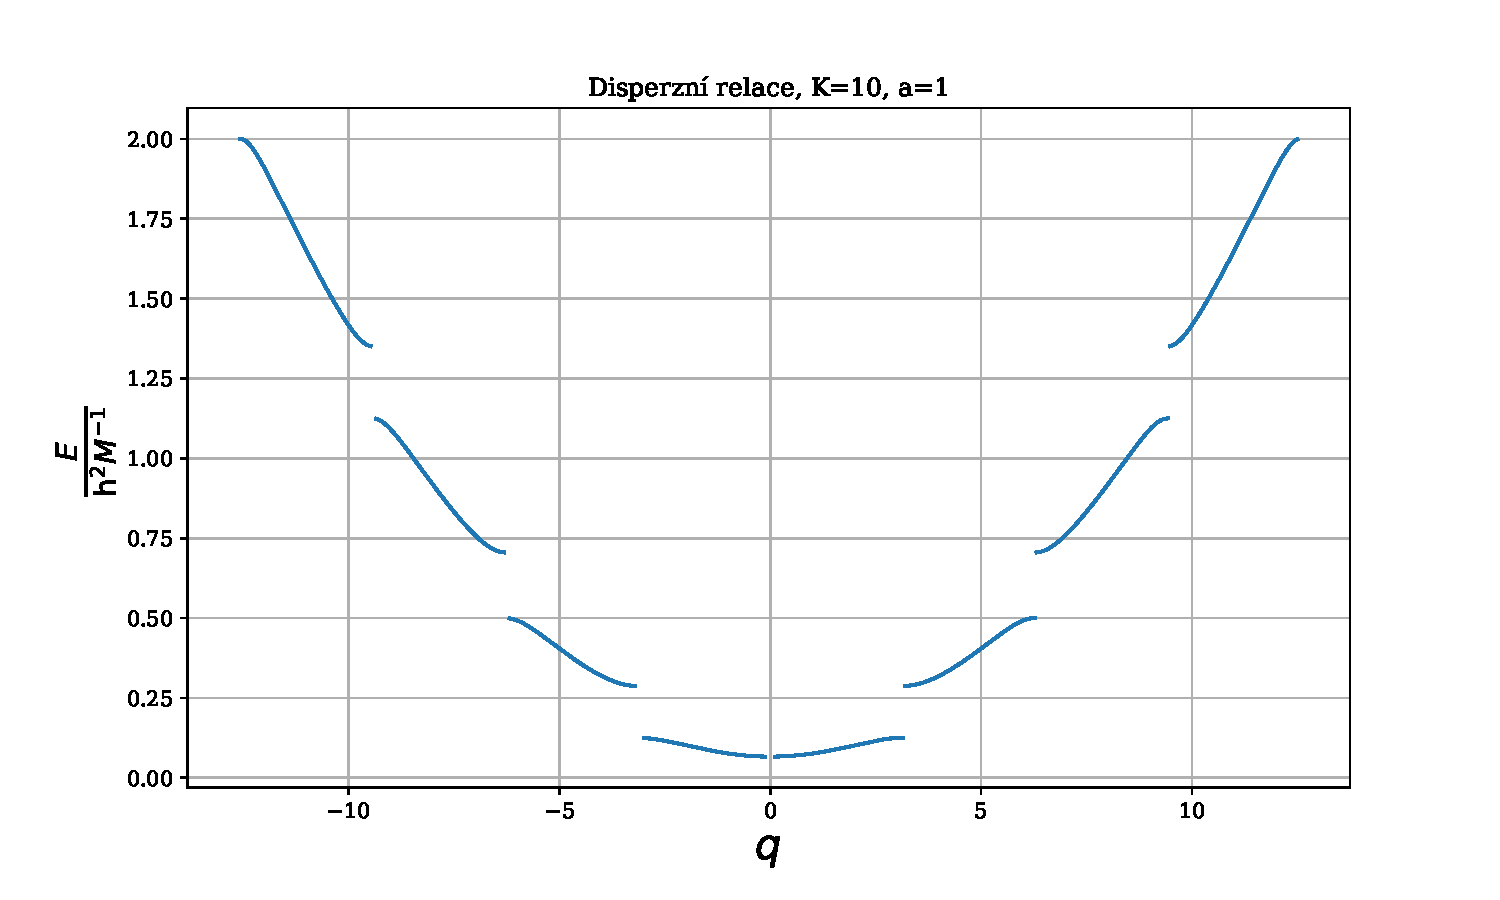
\includegraphics[scale=0.7]{disperzni10.pdf}
    \label{}
\end{figure}

\pagebreak

Pro vypočtení derivace využijeme implicitní funkci. Vztah $\tilde{E}(q)$ vyjádřený jako implicitní funkce má tvar:
\begin{gather*}
    \Phi_K(q, \tilde{E}) =
    \cos{qa} - \theta_K(t(\tilde{E})).
\end{gather*}
Derivace $\tilde{E}$ je potom
\begin{gather*}
    \dd{\tilde{E}}{q}(q(t)) =
    - \frac{\pd{\Phi}{q}(q(t), \tilde{E}(t))}{\pd{\Phi}{q}(q(t), \tilde{E}(t))} =
    - \frac{a \sin aq(t)}{\theta_K'(t) \; t'(\tilde{E}(t))}
    = \frac{4 \pi a^{2} t^{3} \sin{\left(a q(t) \right)}}{- 2 \pi K a t \cos{\left(2 \pi a t \right)} + K \sin{\left(2 \pi a t \right)} + 8 \pi^{2} a^{2} t^{2} \sin{\left(2 \pi a t \right)}}.
\end{gather*}
Pro grupovou rychlost $v_\const{g}$ platí:
\begin{gather*}
    v_\const{g}(q) = \frac{1}{\hbar} \dd{E}{q} = 2 \pi \frac{\const{h}}{M} \dd{\tilde{E}}{q}
\end{gather*}
Veličinu $\tilde{v}_\const{g}$ (opět podělenou konstantami) tedy můžeme v závislosti na $q$, resp. $E$ parametrizovat:
\begin{gather*}
    \phi_q(t) = \mat{
        q_K(t) \\[7pt]
        2 \pi \dd{\tilde{E}}{q}\hspace{-3pt}(q(t))
    },
    \hspace{3em}
    \phi_E(t) = \mat{
        \tilde{E}(t) \\[7pt]
        2 \pi \dd{\tilde{E}}{q}\hspace{-3pt}(q(t))
    }.
\end{gather*}
\begin{figure}[h!]
    \centering
    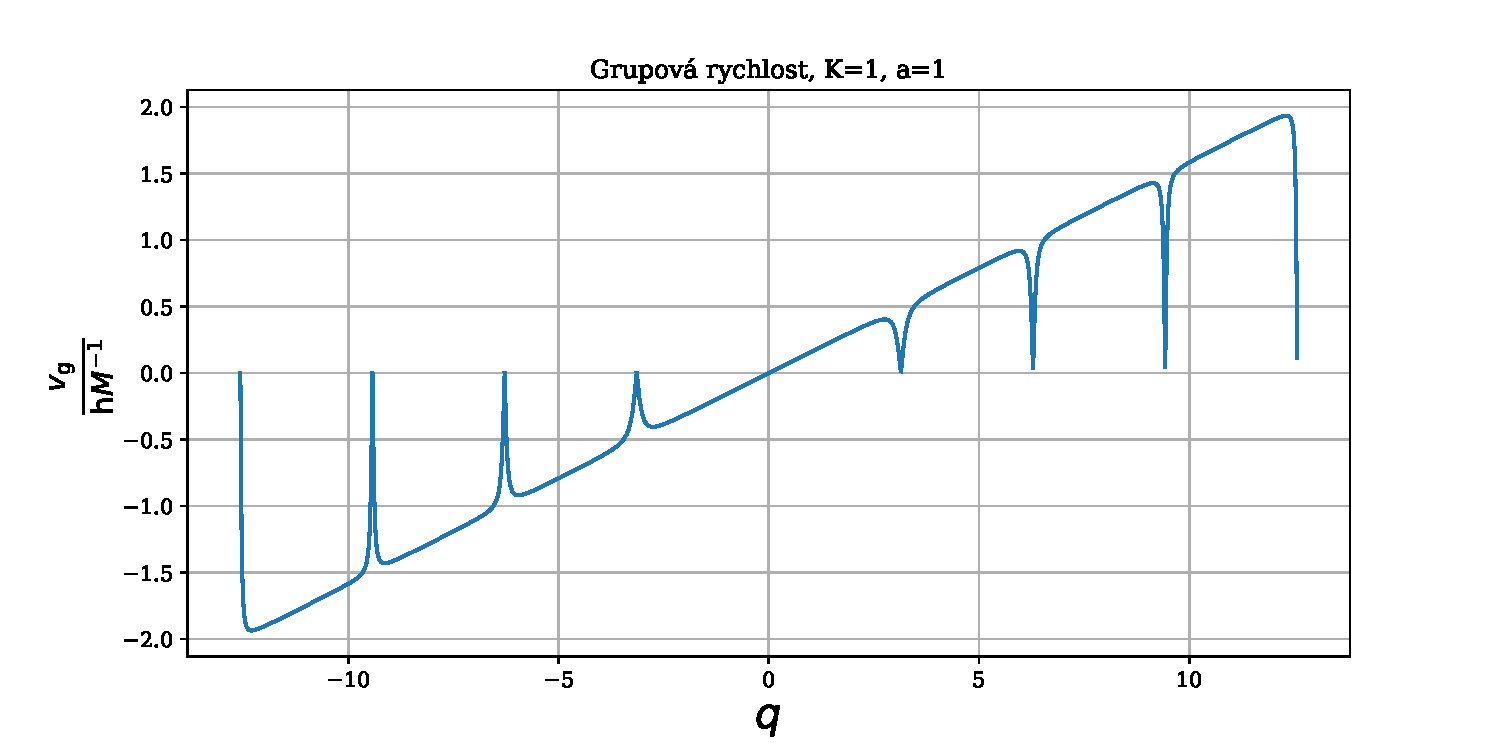
\includegraphics[scale=0.65]{grupova1_q.pdf}
    \label{}
\end{figure}

\begin{figure}[h!]
    \centering
    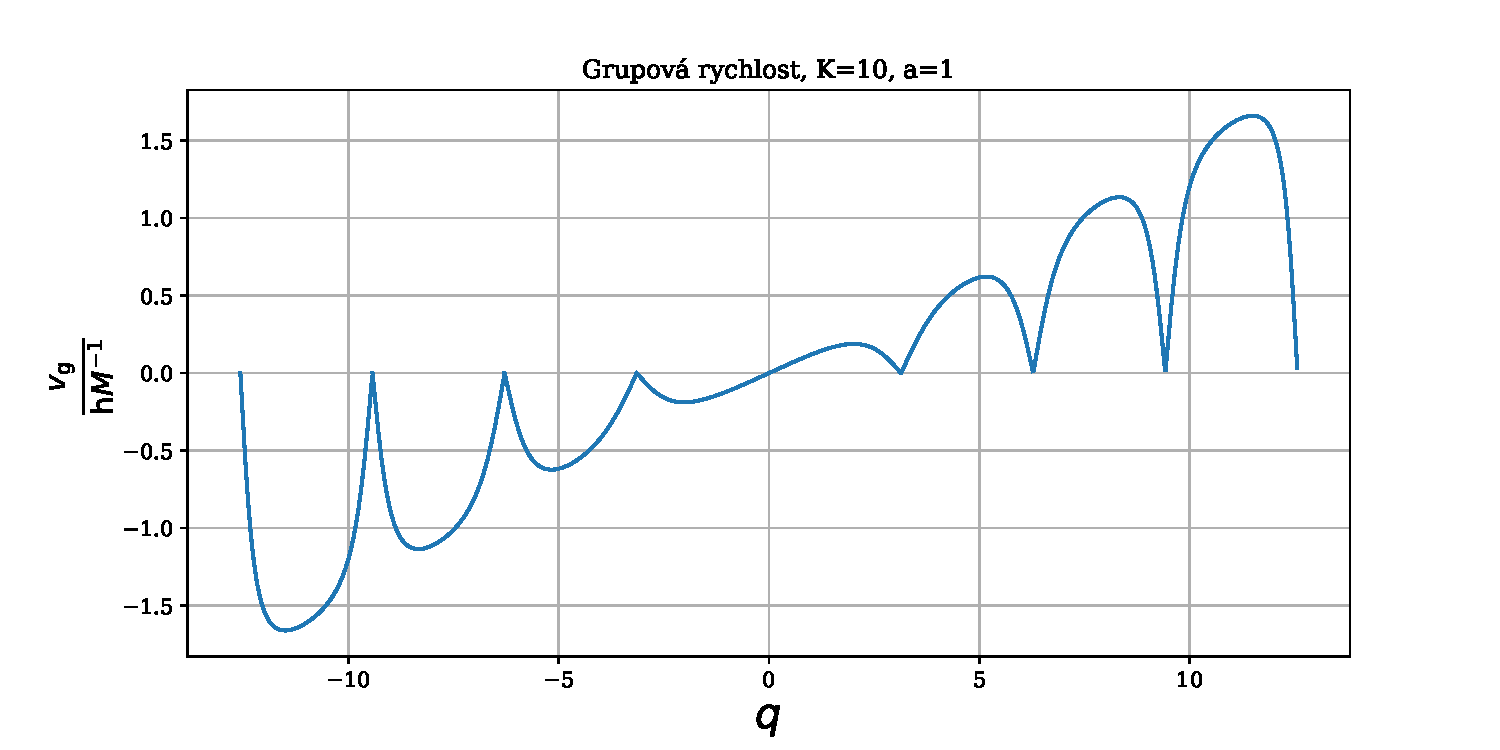
\includegraphics[scale=0.65]{grupova10_q.pdf}
    \label{}
\end{figure}

\begin{figure}[h!]
    \centering
    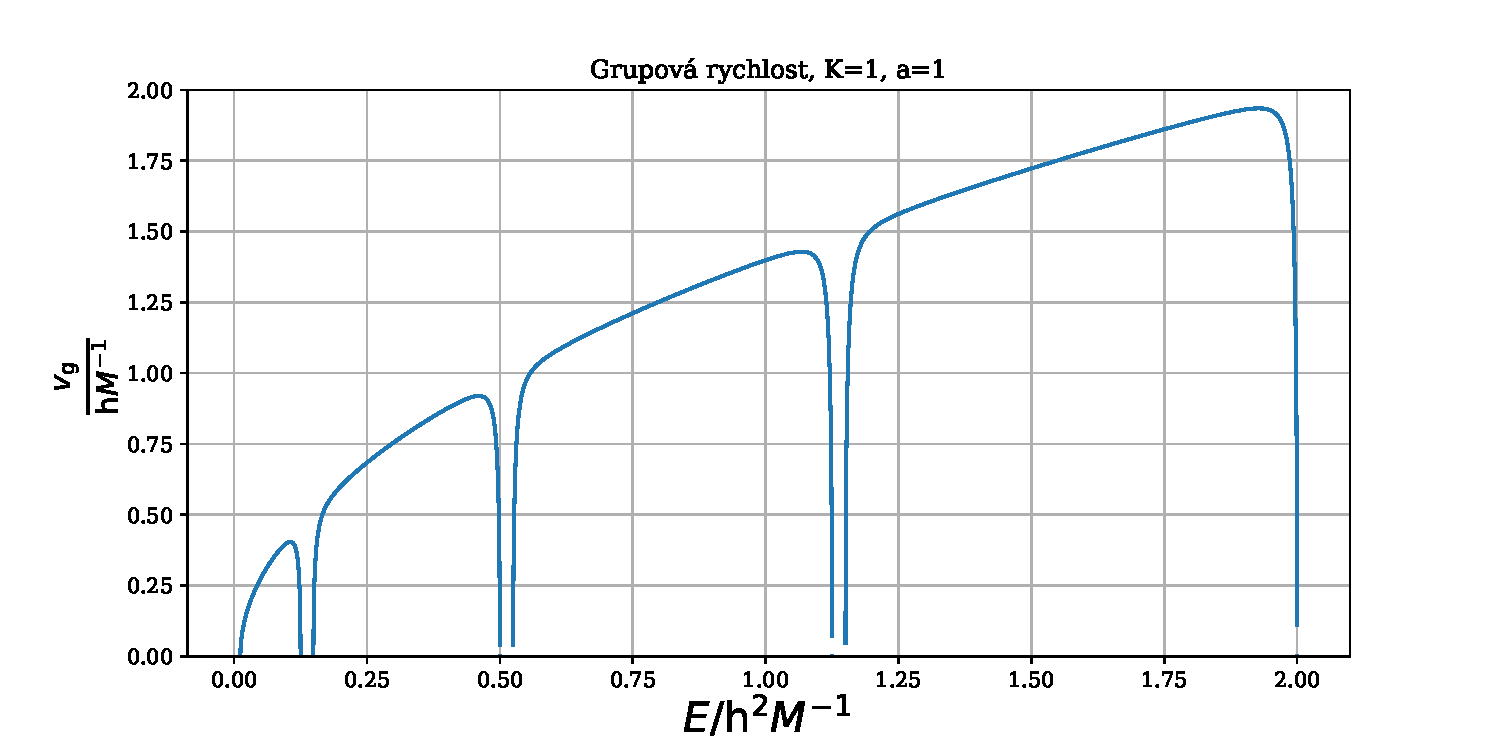
\includegraphics[scale=0.65]{grupova1_E.pdf}
    \label{}
\end{figure}

\begin{figure}[h!]
    \centering
    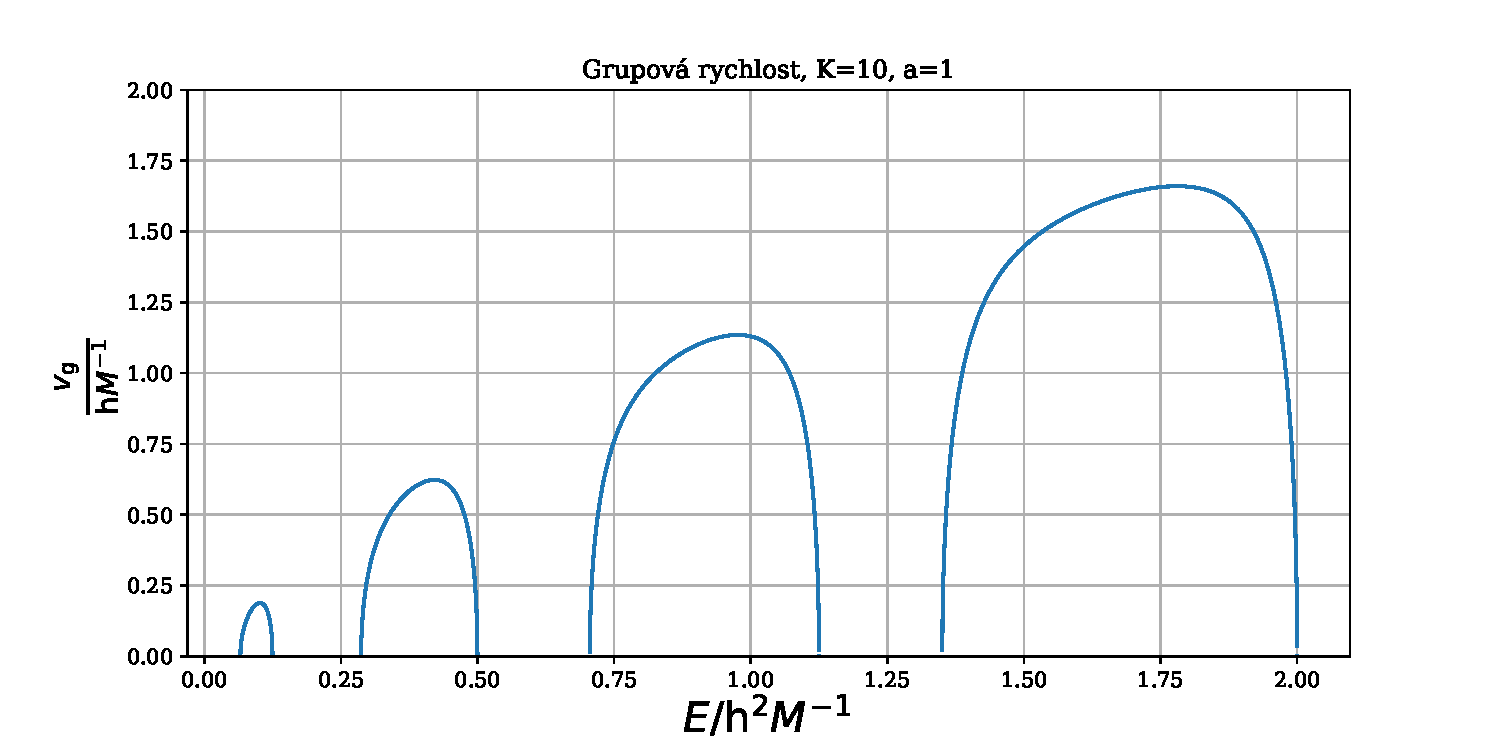
\includegraphics[scale=0.65]{grupova10_E.pdf}
    \label{}
\end{figure}

\subsection{Řešení pro $E<0$}

Pro záporné energie máme podle Blochova teorému:
\begin{align*}
    \psi_I &= \e{\i q x} \left( A \e{-\i q x} \e{kx} + B \e{-\i q x} \e{-kx} \right), \\
    \psi_{II} &= \e{-\i q a} \left( A \e{k(x+a)} + B \e{-k(x+a)} \right).
\end{align*}
Aplikujeme-li nyní slepovací podmínky, získáme:
\begin{align*}
    \psi_{II}(0-) &= \psi{I}(0+) \\
    \e{-\i q a} \left( A \e{ka} +  B \e{-ka}\right) &= A + B
    \\[10pt]
    \psi_{II}'(0-) - \psi_I'(0+) &= - K(A+B) \\
    \e{-\i q a}\left( Ak\e{ka} - B\e{-ka} \right) -kA + kB &= -K(A+B)
\end{align*}
Získáme tedy lineární soustavu dvou rovnic, po převedení do maticové podoby:
\begin{gather}
    \mat{
        \e{-\i qa + ka} - 1 &
        \e{-\i qa - ka} - 1 \\
        k\left(\e{-\i qa + ka} - 1\right) + K &
        -k\left(\e{-\i qa - ka} - 1\right) + K
    }
    \mat{A \\ B} = 0
    \label{maticova-AB}
\end{gather}
Podmínka nulovosti determinantu vede na rovnici
\begin{gather*}
    \cos qa = \cosh ak + \frac{K}{2k} \sinh ak
\end{gather*}
Parametrizace bude zjevně téměř stejná, jako pro případ $E>0$, jenom pomocnou funkci $\theta_K(t)$ si předefinujeme:
\begin{gather*}
    \theta_K(t) = \cosh(2\pi t) + \frac{K}{2k} \sinh(2\pi t).
\end{gather*}
Nakonec ještě normalizujeme vlnovou funkci:
\begin{align*}
    \int_0^a |\psi(x)|^2 \d{x} &=
    \int_0^a \left( A\e{2kx} + 2AB + B\e{-2kx} \right) \d{x} =
    \left[ \frac{A}{2k} \e{2kx} + 2ABx - \frac{B}{2k} \e{-2kx}\right]_0^a
    \\
    &= \frac{A}{2k} \left( \e{2ka} - 1 \right) + 2aAB + \frac{B}{2k} \left( 1 - \e{-2ka} \right)
    = 1
\end{align*}
Tato rovnice společně s \eqref{maticova-AB} stačí k určení koeficientů $A, B$ pro konkrétní hodnoty $q, K, a$.

\begin{figure}[h!]
    \centering
    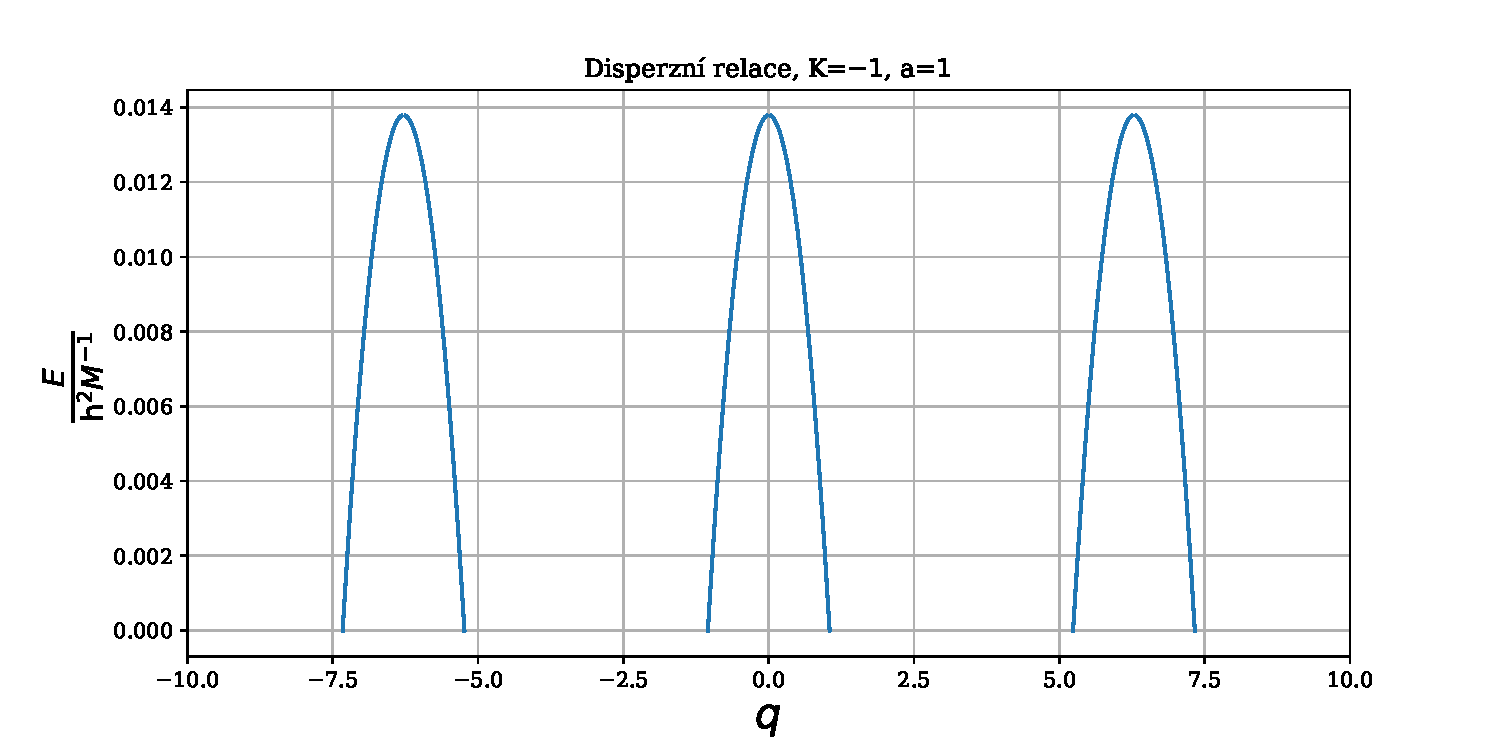
\includegraphics[scale=0.65]{disperzni-1_neg.pdf}
    \label{}
\end{figure}

\begin{figure}[h!]
    \centering
    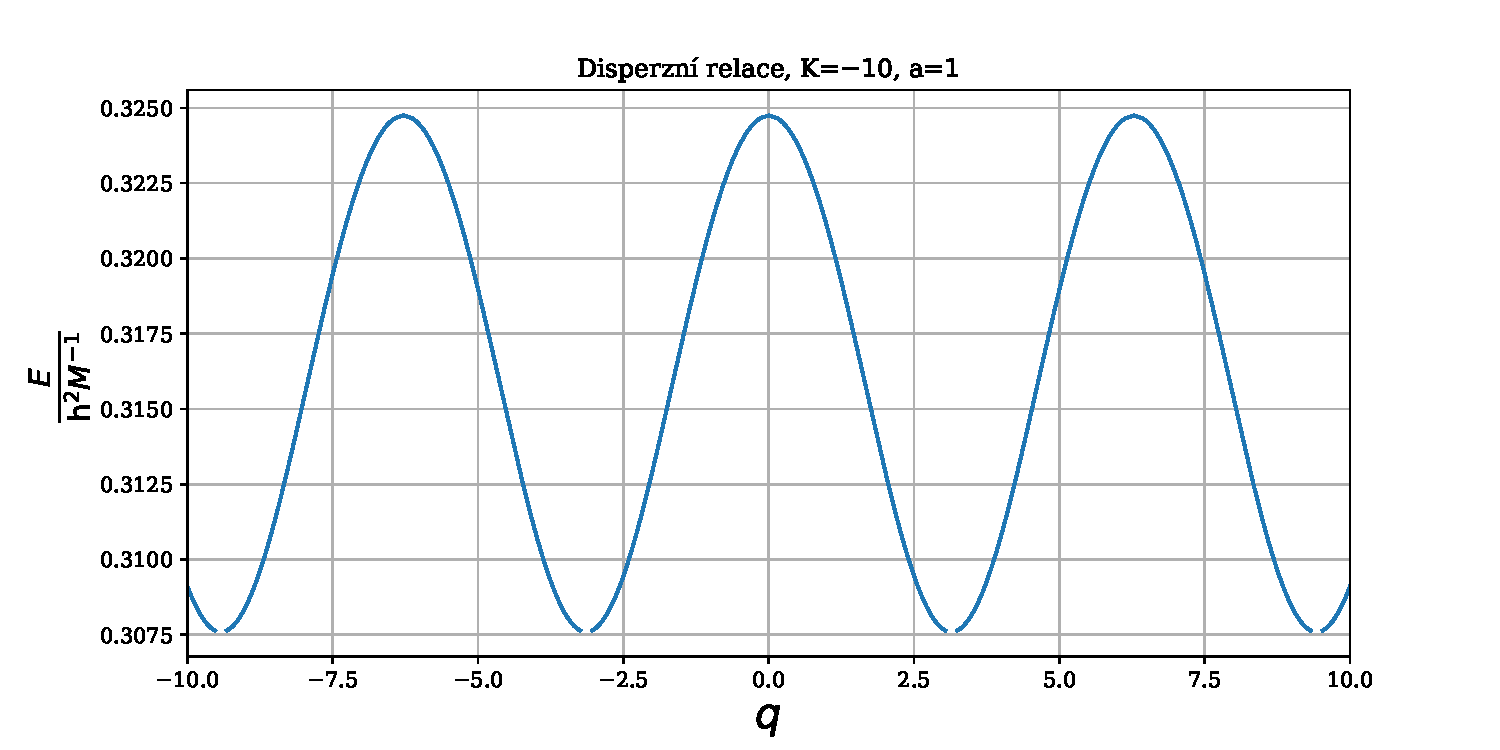
\includegraphics[scale=0.65]{disperzni-10_neg.pdf}
    \label{}
\end{figure}

\end{document}